\documentclass{memoir}
\usepackage{lmodern}
\usepackage[utf8]{inputenc}
\usepackage[italian]{babel}
\usepackage{amsmath}
\usepackage{graphicx}

\graphicspath{{./draws/}}

%\title{How to write a Report\\ for the Project of Distributed Systems}
\title{Progetto di Sistemi Distribuiti}

\author{Dott. Diego Borsoi\\Dott. Filippo Callegari\\ DMIF, University of Udine,
	   Italy}

\date{Version 0.1, \today}

\begin{document}


%\begin{titlingpage}
\maketitle
%\begin{abstract}
%The aim of this document is to describe how to write a report for the project-exam
%	   for the course Distributed Systems, at the University of Udine.
%It is also a guideline for the development of the project itself.
%
%This document is very brief and succint, and it is by no means comprehensive of
%	   all
%	   the informations that should be given about a software project. You are invited
%	   to
%	   supplement these guidelines as needed to best describe your work.
%\end{abstract}
%\end{titlingpage}

\chapter{Introduzione}\label{ch:intro}

Il progetto in questione riguarda la creazione di un sistema distribuito per la comunicazione
	   fra dispositivi all'interno di una rete sparsa, tramite l'utilizzo di eventi.

\section{Descrizione del problema}

Ogni dispositivo corrisponde ad un nodo della rete ed è caratterizzato da:
\begin{itemize}
\item \textbf{Id} : numero univoco del nodo.
\item \textbf{Stato} : tupla di variabili che rappresentano delle specifiche caratteristiche
	   del nodo (es. temperatura di un sensore, stato di accensione di una termocoppia,
	   ecc).
\item \textbf{Regole} : insieme di regole del tipo ECA (Event Condition Action) che
	   possono attivarsi a seguito di un evento inviato al nodo. Queste regole possono
	   essere
	   di due tipi: locali, l'azione modifica solamente lo stato del nodo in cui si
	   attiva,
	   oppure globale, l'azione viene inviata a tutti i nodi della rete perché venga
	   letta
	   ed, in caso la valutazione della guardia associata sia positiva, eseguita.
\center$\{event;~condition;~action~|~\text{if}~guard~\text{then}~action\}$
\end{itemize}

Lo stato della rete si evolverà ogni qual volta un evento verrà attivato, andando
	   a sua volta ad innescare eventuali nuovi eventi e creando quindi una sequenza
	   di
	   azioni a cascata.

\section{Struttura dell'implementazione}

La rete in questione ha una struttura a mesh sparsa (cioè ogni nodo sarà al più
	   connesso a un numero di nodi molto basso, rispetto alla totalità).
I nodi sono idempotenti in modo tale da avere un sistema fortemente decentralizzato.
Le varie comunicazioni fra i nodi sono eseguite al di sopra di connessioni TCP, in
	   tal modo possiamo garantire la consegna di ogni messaggio nell'ordine prestabilito.
Per quanto concerne invece le comunicazioni riguardanti il sistema di $heartbeat$
	   (\ref{heartbeat}), queste vengono eseguite utilizzando connessioni UDP.

\section{Trasparenze}\label{Trasparenze}

Di seguito sono descritte le trasparenze che concergono e sono implementate dal sistema:

\begin{description} 
\item[Trasparenza ai fallimenti:] nel momento in cui un nodo fallisce/si disconnette,
	   il resto della rete continua a funzionare normalmente.
\item[Trasparenza alla scalabilità:] la rete può espandersi in dimensione senza
	   che il funzionamento dei nodi vari.
\item[Trasparenza alla mobilità:] un nodo può spostarsi all'interno della rete
	   senza che il funzionameto suo e degli altri nodi vada a modificarsi.
\end{description}

\section{Algoritmi}

Il sistema implementa solamente due algoritmi:
\begin{itemize}
\item \textbf{Flooding Algorithm:} viene usato per la comunicazione di un'azione
	   a tutta la rete nel momento in cui in un nodo una regola globale viene attivata.
\item \textbf{Lamport clock (modificato):} viene utilizzata una versione modificata
	   del Lamport clock per identificare i vari $flood$ eseguiti; questo clock viene
	   incrementato
	   solamente dall'invio (o ricezione) di un messasggio, e non dalle azioni interne
	   ad
	   un nodo.
\end{itemize}

Il sistema non implementa particolari algoritmi essendo che si vuole realizzare una
	   rete distribuita dove ogni nodo conosce esclusivamente i vicini ed evolve il
	   suo
	   stato solamente a causa di eventi ricevuti tramite dei messaggi.

\section{Testing}

Per testare il sistema verrà utilizzata un'entità $Ambiente$, la quale simulerà:
	   
\begin{itemize}
\item la creazione iniziale della rete, caricando da dei file appositi la struttura
	   degli stati, la lista di regole e la conformazione della rete
\item la scoperta di nuove connessioni
\item variazioni di variabili legate all'ambiente (es. temperatura registrata da
	   un sensore)
\item fallimenti di nodi
\item ritardi nell'invio di messaggi fra nodi
\end{itemize}

Ogni modulo verrà testato singolarmente ed infine verranno eseguiti dei test completi
	   del sistema.

\section{Piano di sviluppo}

Le future fasi di sviluppo seguiranno il seguente ordine:
\begin{enumerate}
\item Riunione con il committente per convalidare la risoluzione del problema
\item Implementazione ambiente virtuale per la gestione dei nodi 
\item Implementazione della struttura del nodo
\item Implementazione sistema $heartbeat$
\item Implementazione del sistema algoritmico
\item Test totale
\item Validazione
\end{enumerate}


%\section{Istruzioni}
%In this chapter you describe the main problem, and an idea of the solution.
%It is not necessary to be very detailed or formal, but it is important to explain
%	   which are the main aims and issues from the point of view of Distributed Systems:
%\begin{itemize}
%\item A description of the application.
%\item The overall structure of the implementation: how resources are deployed, which
%	   are the players, the r\^oles.
%\item The distributed system features (and the transparencies) and algorithms you
%	   intend to implement.
%\item Your plan for testing the system.
%\item A schedule for how you plan to carry out your design and implementation
%\end{itemize}

\chapter{Analisi}\label{ch:analisi}

In questo capitolo vengono descritti nel dettaglio requisiti funzionali e non funzionali
	   della soluzione proposta.

\section{Requisiti Funzionali}

I requisiti funzionali individuati sono:
\begin{itemize}
\item \textbf{Categorizzazione di un nodo:} ogni nodo ha un tipo il quale ne identifica
	   lo stato e le sue regole;
\item \textbf{Modifica delle regole di un nodo:} ogni tipo di nodo può avere le
	   sue regole, codificabili attraverso la programmazione dello stesso;
\item \textbf{Modifica dello stato di un nodo:} ogni evento permette di avere o degli
	   \textit{effetti locali} o degli \textit{effetti globali}:
	\begin{itemize}
	\item \textit{\textbf{effetti locali}}: la regola va a modificare lo stato interno;
	\item \textit{\textbf{effetti globali}}: la regola può modificare lo stato delle
	   variabili interne, e può generare un evento sugli altri nodi;
	\end{itemize}
\item \textbf{Aggiunta dinamica di un nodo:} un nodo può essere aggiunto alla rete
	   in qualsiasi momento senza perturbarne la dinamicità, limitando l'aggiornamento
	   ai vicini a cui si collega.
\item \textbf{Esecuzione di un'azione ricevuta dai vicini:} nel momento in cui un
	   nodo riceve un messaggio dai propri vicini esso va a verificare la soddisfacibilità
	   della guardia (se presente) e nel caso di una valutazione positiva viene eseguita
	   l'azione associata, andando quindi a modificare il proprio stato.
\item \textbf{Attivazione di una regola:} ogni qual volta avviene un cambiamento
	   nello stato di un nodo, viene eseguito un controllo delle regole, per vedere
	   se gli
	   eventi generati possano attivare una o più regole del nodo; nel caso in cui
	   una
	   regola venga attivata, in base al tipo (locale o globale) viene portata a termine
	   l'azione corrispondente.
\end{itemize}

\section{Requisiti Non Funzionali}

I requisiti non funzionali individuati sono:
\begin{itemize}
\item \textbf{Decentralizzazione:} nessun nodo ha il controllo dell'ordine degli
	   eventi, grazie al fatto che ogni nodo è idempotente;
\item \textbf{Tolleranza ai guasti:} poiché tutti i nodi sono idempotenti, nel momento
	   in cui un nodo si scollega dalla rete, la rete rimanente continua ad operare
	   normalmente;
\item \textbf{Etereogenità:} fintanto che i nodi aggiunti utilizzano il protocollo
	   descritto, qualunque nodo di qualunque tipo (hardware o categoria) potrà essere
	   aggiunto alla rete;
\item \textbf{Scalabilità:} l'aggiunta dinamica dei nodi alla rete permette di scalare
	   orizzontalmente con estrema facilità;
\item \textbf{Trasparenze:} le trasparenze implementate sono quelle descritte al
	   capitolo precedente (paragrafo \ref{Trasparenze}).
\end{itemize}

%\chapter{Analysis}\label{ch:analysis}
%
%In this chapter, we describe in detail functional and non-functional requirements
%	   of a solution for the problem.
%
%\section{Functional requirements}
%Which functions must be offered to users / other programs?  Which are the input
%	   data and the output data? Which is the expected effect? 
%
%\section{Non functional requirements}
%Everything about mode and transparencies: availability, mobility, security, fault
%	   tolerance, etc.
%
%Are there execution time bounds? Minimum data rates?
%
%If requested, specific platforms/languages/middlewares requirements for the implementation
%	   can be decided here. (E.g.: if the project is on a SOA, we may request that
%	   functions
%	   are offered via SOAP or RESTful services). 



\chapter{Progetto}\label{ch:progetto}

In questo capitolo vengono descritti in modo più approfondito l'achitettura del
	   progetto, i moduli, i protocolli e gli algoritmi utilizzati.

\section{Architettura logica}

Essendo tutti i nodi costruiti al medesimo modo, di seguito presentiamo la struttura
	   di uno singolo di essi. 

\begin{figure}[h]
\makebox[\linewidth][c]{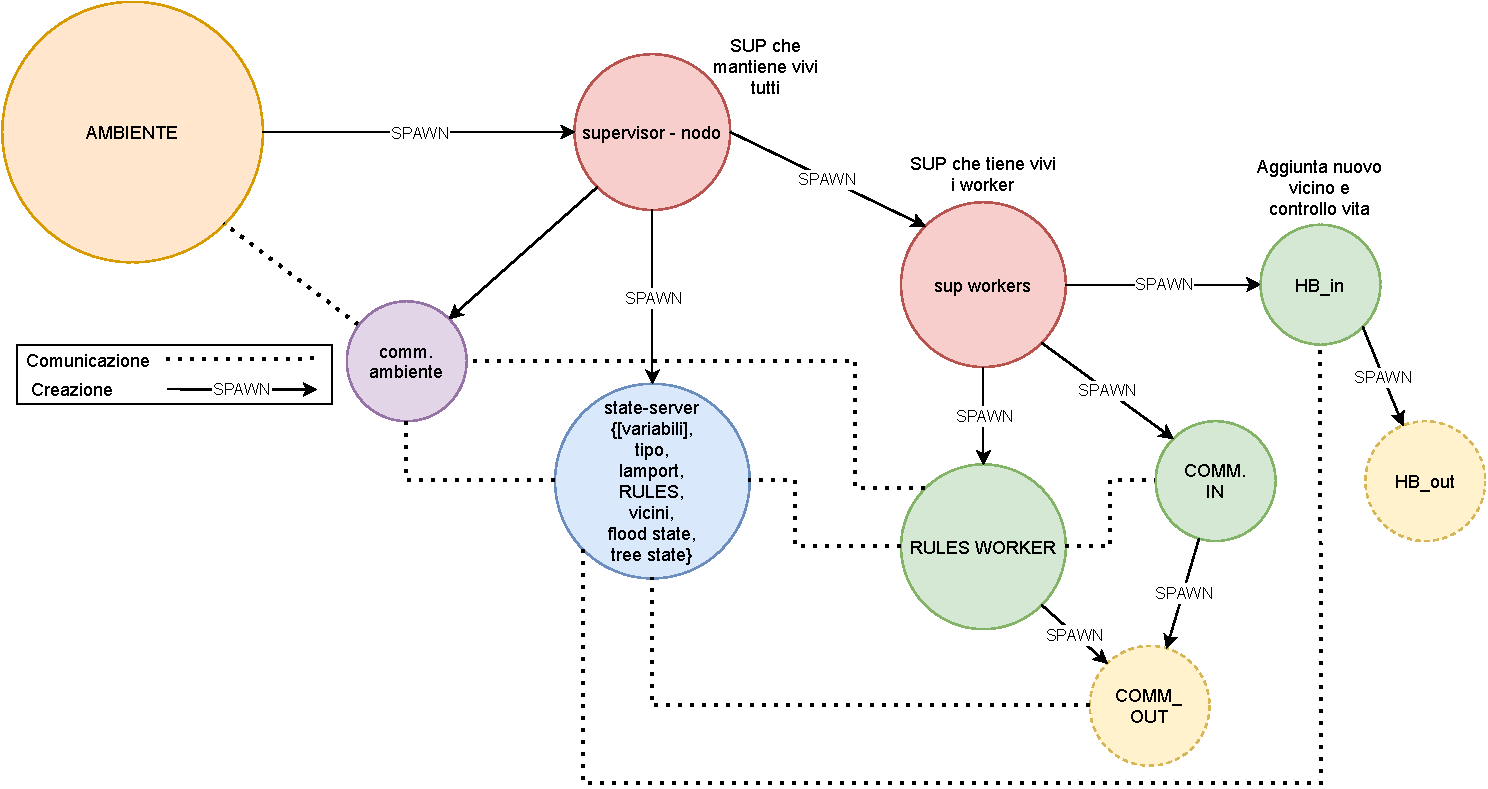
\includegraphics[scale=0.6]{draw_nodeworker.pdf}}
%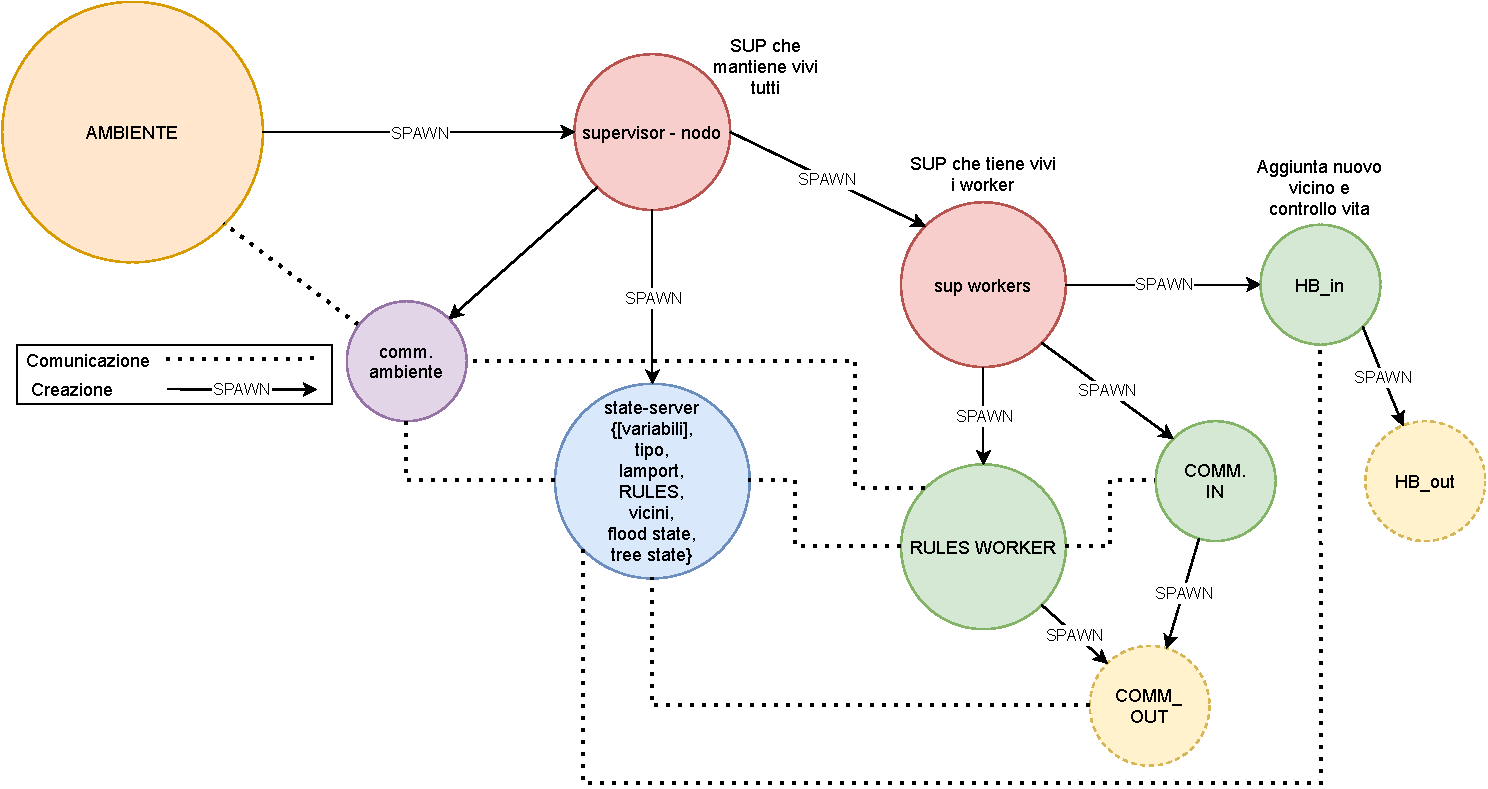
\includegraphics[scale=0.6]{draw_nodeworker.pdf}
%\centering
\caption{Struttura gerarchica dei moduli di un nodo e visualizzazione delle connessioni
	   fra di essi.}
\label{img:struttura_nodo}
\end{figure}

Come si può vedere dalla figura \ref{img:struttura_nodo}, ogni nodo è formato dai
	   seguenti moduli:
\begin{itemize}
	\item \textbf{Supervisor nodo:} modulo che cerca di manterene sempre operativi gli
	   altri moduli interni. Se questo componente si riavvia equivarrebbe ad un riavvio
	   del nodo, e quindi la conseguente perdita della modifica agli stati interni.
	   I moduli
	   da lui controllati sono:
	\begin{itemize}
	\item \textbf{State server:} questo modulo manterrà tutte le variabili locali al
	   nodo, che verranno modificate durante l'operatività dello stesso. Queste variabili
	   sono:
		\begin{itemize}
		\item stato del nodo;
		\item lista delle regole associate al nodo;
		\item tipo del nodo;
		\item stato delle waves; %sia clock che cose precedenti
		\item informazioni sui nodi vicini;
		\item id univoco del nodo;
		\end{itemize}
	\item \textbf{Supervisor dei workers:} modulo che si occupa di gestire i moduli
	   a lui dipendenti, riavviandoli in caso di ``crash". Questi sono:
		\begin{itemize}
		\item \textbf{heartbeat sense:} si occupa di controllare la ``vitalità" dei vicini
	   e di istanziare le connessioni con essi;
		\item \textbf{communication in:} si occupa di gestire tutti i messaggi in ingresso
	   relativi al nodo in questione;
		\item \textbf{rules worker:} si occupa di applicare le azioni ricevute dai nodi
	   vicini ed eventualmente eseguire una delle regole a lui locali al momento dell'attivazione;
	   lui si occuperà anche di propagare le regole che generano degli eventi verso
	   gli
	   altri nodi, interpellando il modulo ``\textit{communication out}'' 
	  (modulo apposito per l'invio dei messaggi ai nodi vicini).
		\end{itemize}
	\end{itemize}
\end{itemize}

Come è stato accennato in precedenza verrà sviluppato un ulteriore modulo chiamato
``\textbf{\textit{Ambiente}}": questo modulo permette di simulare le interazioni
	   che avverrebbero nel mondo reale. Nel dettaglio, le funzionalità del modulo
	   sono:
\begin{itemize}
	\item il "discovery" dei vicini;
	\item cambiamento delle variabili non dipendenti dalle regole (temperatura dell'ambiente/GPS/...);
	\item simulazioni di disservizi di rete;
	\item simulazione di guasti (temporanei o non) di un nodo;
	\item topologia della rete.
\end{itemize}
Dal punto di vista del nodo ci troviamo quindi costretti ad aggiungere un ulteriore
	   modulo fittizio (\textbf{\textit{comunicazione ambiente}}) per permettere la
	   comunicazione
	   con l'ambiente.

\section{Protocolli ed algoritmi}

Di seguito verranno descriti nel dettaglio i vari protocolli ed algoritmi utilizzati.

\subsection{Controllo e attivazione delle regole}

Nel momento in cui il sistema riceve un'azione da eseguire (dopo aver controllato la validità e che appartenga ad una wave non ancora ricevuta) si innesca la seguente serie di azioni:
\begin{enumerate}
\item il modulo \textit{communication IN} invia l'azione da eseguire al modulo \textit{rules worker};
\item quest'ultimo utilizza una funzione dello \textit{state server} per modificare lo stato del nodo in accordo all'azione ricevuta;
\item il \textit{rules worker} esegue quindi un controllo sulle regole andando ad identificare quali possono essere attivate dalla modifica appena eseguita;
\item per ciascuna regola che viene attivata viene testata la condizione e in caso di risultato positivo:
\begin{itemize}
\item se la regola è del tipo \textit{locale}, viene eseguita l'azione associata
\item se invece la regola è del tipo \textit{globale}, viene eseguita l'azione associata (in caso di guardia con valutazione positiva) e viene passata ad un processo di \textit{communication OUT}, istanziato appositamente, che genera una nuova wave di messaggi inviando ai vicini la nuova azione.
\end{itemize}
\end{enumerate}

\subsection{Heartbeat}\label{heartbeat}
L'algoritmo di ``heartbeat'' serve per mantenere consistente lo stato dei vicini
	   di un nodo. Questo infatti controlla la loro vitalità e sarà componente chiave
	   per l'aggiunta di un nuovo nodo.

L'algoritmo si suddivide quindi in due componenti:
\begin{itemize}
	\item \textit{ECHO}: similmente al protocollo ICMP, si fa una richiesta di echo
	   al vicino. Se questa ``\textit{ECHO\_RQS}" andrà a buon fine, il primo nodo che
	   istanzia una richiesta di ``\textit{ECHO}" richeverà un pacchetto di ``\textit{ECHO\_RPL}".
	   Definiamo come $\tau$ il tempo che intercorre tra un messaggio di \textit{ECHO} ed
	   un'altro. Se un nodo non rispondesse entro $2\tau$ ad una \textit{ECHO\_RQS}, questo
	   verrà considerato come non più collegato. Ogni \textit{ECHO\_RPL} conterrà il ``Lamport"
	   attuale del vicino.
	\item \textit{ADD\_NEW\_ND}: similmente al protocollo DHCP, nella fase di aggiunta
	   di un nodo alla rete, il nuovo nodo si annuncia al suo vicino ``fisico'', chiedendo
	   le informazioni essenziali per poter partecipare attivamente alla rete. Questo sarà
	   spiegato più in dettaglio nella prossima sezione.
\end{itemize}

\begin{figure}[h]
\centering
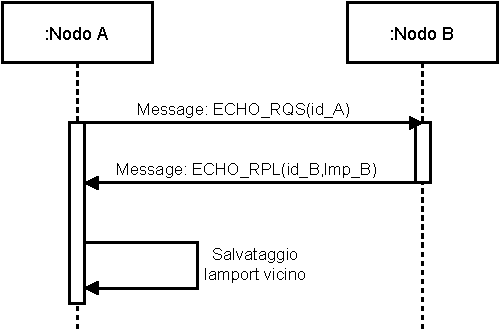
\includegraphics{HeartbeatDiagram.pdf}
\caption{Sequence diagram dei messagi usati per il sistema di \textit{heartbeat}.}
\label{img:heartbeat}
\end{figure}

\subsection{Aggiunta di un nuovo nodo}
L'aggiunta di un nodo è una parte complicata del sistema: bisogna tener conto della
	   possibilità che la rete si partizioni. Questo si può verificare nel caso in cui
	   un nodo si riavvii. Il partizionamento della rete è visto come caso particolare
	   di aggiunta di un nodo alla rete.

L'aggiunta di un nuovo nodo si compone dei seguenti passi:
\begin{enumerate}
	\item \textit{ADD\_NEW\_ND}: il nuovo nodo manda la richiesta di aggiunta alla rete
	   a tutti i suoi vicini inviando il proprio id;
	\item \textit{ADD\_NEW\_NB}: il nodo che deve aggiungere il nuovo nodo risponde
	   con un messaggio contenente $(lamport,id)$.
\end{enumerate}
A questo punto, una volta che per ogni vicino ho i suoi parametri di lamport, i casi
	   possibili sono 2:
\begin{enumerate}
	\item \textbf{tutti i nodi hanno medesimo lamport:} imposto il mio lamport al lamport
	   comune;
	\item \textbf{esiste un lamport massimo:} imposto il mio lamport al valore massimo,
	   e rispondo con \textit{UPD\_LMP} a tutti i miei vicini che non hanno il lamport al
	   massimo. Questi a loro volta manderanno a tutti i loro vicini, con lamport diverso
	   da quello scelto, il nuovo valore.
\end{enumerate}

\begin{figure}[h]
\makebox[\linewidth][c]{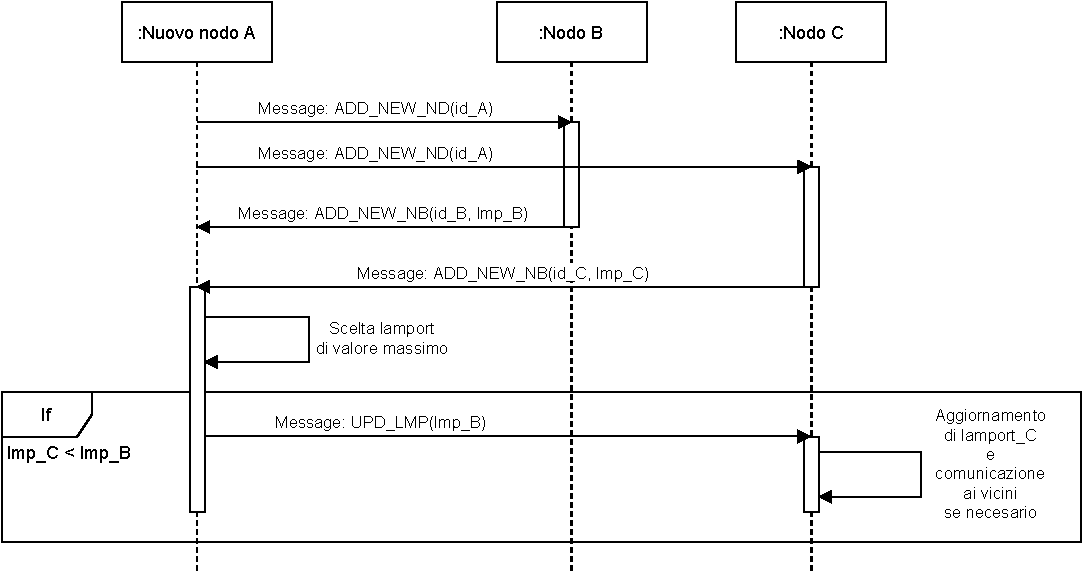
\includegraphics[scale=0.9]{NewNodeDiagram.pdf}}
\caption{Sequence diagram dei messagi usati per laggiunta di un nuovo nodo alla rete.}
\label{img:newnode}
\end{figure}

\subsection{Algoritmo: Flooding}
Ogni qual volta si crea una regola che genera un evento "globale", ogni nodo spedirà
	   ai suoi vicini un messaggio contenenta un'azione da eseguire. Questi, una volta ricevuto,
	   aggiorneranno il loro "wave count" (tenuto dal Lamport modificato, spiegato successivamente),
	   e passerà all'esecuzione dell'istruzione condizionata contenuto nel messaggio. Al
	   fine di evitar la presenza di messaggi vecchi nella rete, ogni messaggio conterrà
	   la coppia $(lamport,id\_gen)$: questo verrà salvato localmente nel nodo ricevente,
	   e verrà mantenuto in memoria al fine di verificare se un messaggio ricevuto non
	   è già stato eseguito. Ogni nodo quindi spedirà una copia del messaggio a tutti
	   i suoi vicini (a patto non l'abbia già ricevuto in passato), meno a quello da cui
	   l'ha ricevuto. Queste strategie applicate faranno si che i messaggi circolanti nella
	   rete siano il minor numero possibile, e nell'eventuale creazioni di cicli nella rete,
	   dovuta alla topologia della stessa, siano soppressi alla prima occasione utile.

\begin{figure}[h]
\makebox[\linewidth][c]{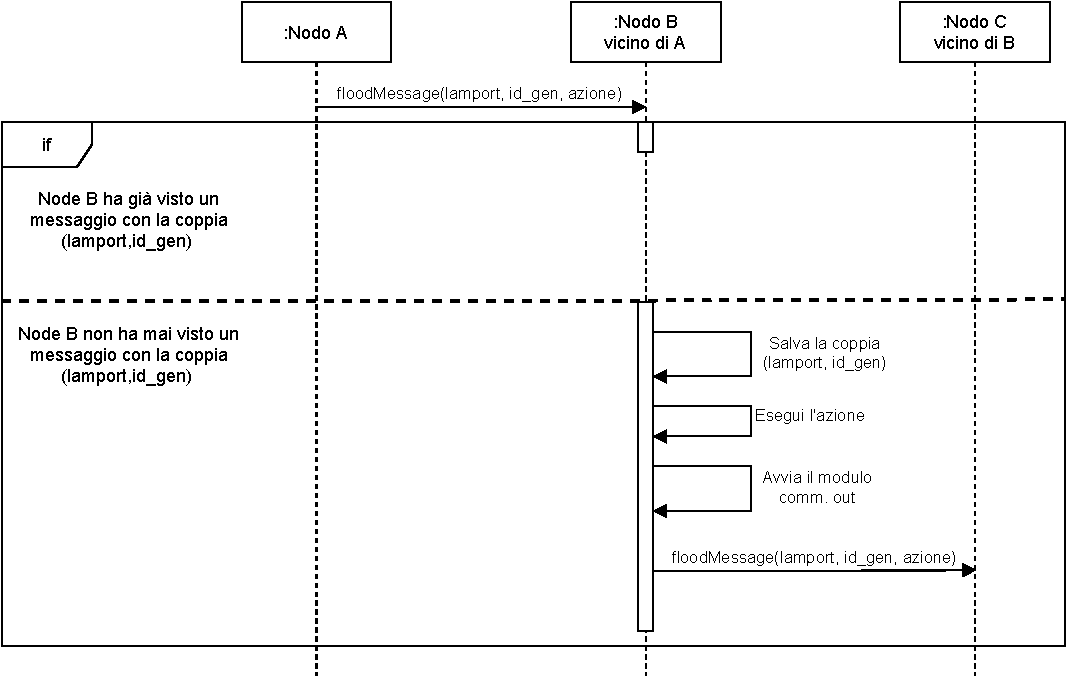
\includegraphics[scale=0.8]{FloodDiagram.pdf}}
\caption{Sequence diagram dei messaggi usati per l'algoritmo di flooding.}
\label{img:flooding}
\end{figure}

\subsection{Algoritmo: Lamport modificato}
Il ``Clock di Lamport" ci permette di dare una certa conseguenza temporale alle azioni.
	   Questo sarà un numero intero crescente, ed identificherà ogni wave generata. Alla
	   generazione di una wave ogni nodo userà il suo lamport interno, incrementato, per
	   identificarla. Questo ci permette, come già abbiamo spiegato, di controllare la
	   propagazione dei messaggi. Sia quindi $Lmp_i$ il lamport della nuova wave ricevuta
	   e $Lmp_n$ il lamport del nodo corrente. Le azioni intraprendibili sono:
\begin{itemize}
	\item $Lmp_i = Lmp_n + 1$: eseguo immediatamente l'azione in essa contenuta ed aggiorno
	   il valore di $Lmp_n$;
	\item $Lmp_i > Lmp_n + 1$: aspetto un preimpostato timeout (es: $5\tau$) prima di
	   eseguire l'azione di $Lmp_i$, in modo tale da poter ricevere le wave mancanti, e
	   quindi mantenere l'ordine causale delle azioni;
	\item $Lmp_i < Lmp_n$: vado ad eseguire l'azione solo nel caso in cui tutte le variabili
	   coinvolte non siano già state modificate da una wave ad essa successiva, cioè con
	   $lamport > Lmp_i$.
\end{itemize}

\section{Architettura fisica e deployment}
Per quanto riguarda l'architettura fisica è necessario l'utilizzo di microcalcolatori,
	   come dei ``Raspberry" o degli ``Arduino". Ogni nodo corrisponderebbe fisicamente
	   ad una di queste schede, avendo quindi la possibilità d'utilizzare più nodi
	   per
	   il medesimo ``apparato".

Non è strettamente necessario l'ausilio di microcalcolatori: potrei concentrare
	   all'interno di un singolo calcolatore più nodi, a patto che siano gestiti in
	   maniera
	   consona. 

Come descritto in precedenza, questi comunicherebbero con protocollo TCP ed UDP,
	   non interessandoci quindi di tutta la rete sottostante.

Visto l'esempio a cui abbiamo pensato, si ritiene ideale l'utilizzo di connessioni
	   wireless.
\section{Piano di sviluppo}
Le \textbf{funzionalità di base} che verranno implementate sono:
\begin{itemize}
	\item comunicazione tra nodi;
	\item sistema di flooding;
	\item sistema di heartbeat;
	\item gestione dell'aggiunta di un nodo alla rete;
	\item gestione del riavvio di un nodo nella rete;
	\item impostazione iniziale dei nodi (ambiente);
	\item programmazione dei nodi;
	\item sistema basico d'esecuzione delle regole.
\end{itemize}
Sono state inoltre individuate le seguenti \textbf{funzionalità avanzate}:
\begin{itemize}
	\item sistema avanzato d'esecuzione delle regole;
	\item salvataggio dello stato del nodo su files interni al controllore;
	\item riprogrammazione dinamica del nodo;
	\item implementazione di un \emph{calculus} locale.
\end{itemize}


%\chapter{Implementation}
%
%Details about the implementation: every choice about platforms, languages, software/hardware,
%	   middlewares, which has not been decided in the requirements.
%
%
%Important choices about implementation should be described here; e.g., peculiar
%	   data structures.


%\chapter{Validation}
%
%Check if requirements from Chapter~\ref{ch:analysis} have been fulfilled.
%Quantitative tests (simulations) and screenshots of the interfaces are put here.


%\chapter{Conclusions}
%
%What has been done with respect to what has been promised in Chapters~\ref{ch:intro}
%	   and \ref{ch:analysis}, and what is left out.

%\appendix
%
%\chapter{Appendix}
%
%In the Appendix you can put code snippets, snapshots, installation instructions,
%	   etc.


%\chapter*{Evaluation}
%Your system will be judged mainly on how it operates as a distributed system. The
%	   primary evaluation will be according to whether your system has the following
%	   attributes:
%\begin{itemize}
%\item  It should be an interesting distributed system, making use of some of the
%	   algorithms we have covered in class for distributed synchronization, replication,
%	   fault tolerance and recovery, security, etc.
%\item The software should be well designed and well implemented, in terms of the
%	   overall architecture and the detailed realization.
%\item You should devise and apply systematic testing procedures, at both the unit
%	   and systems levels.
%\item The system should operate reliably and with good performance, even in the
%	   face of failures.
%\end{itemize}
%Important, but secondary considerations include:
%\begin{itemize}
%\item Time taken to do the project (the sooner the better, but do not miss details
%	   in order to end sooner)
%\item  How nice is the application's appearance: does it have a nice interface or
%	   a compelling visual display?
%\end{itemize}

\end{document}
